\section{Resultados}\label{sec:resultados}

Comandos foram utilizados para a estruturação de ``Corais'', pequenas peças didáticas de, por colagem de materiais da bachianos, recorte por técnica \emph{glitch}\footnote{Aplicação de recortes indeterminados  sobre um material pré existente.}, e readequações de discurso harmônico pós-tonal. Resultados foram possíveis com a implementação da a opção \verb|--CAC| ou \verb|-C|, como no código abaixo. No entanto esta é apenas uma \emph{flag} indicativa que um material será reconfigurado. Inclui, até o momento, a \emph{flag} \verb|--glitch| ou \verb|-g|, que recorta o material fornecido.

\begin{listing}
\begin{minted}[linenos,frame=leftline,fontsize=\footnotesize]{python}
./main.py --show --CAC --composer bach --index bwv1 --glitch 2
./main.py -S -C -c bach -i bwv1 -g 2
\end{minted}
\end{listing}

\subsection{BWV1}\label{sec:bwv1}

Experimentamos uma aplicação de erros no sexto movimento de \emph{Wie schün leucht der Morgenstern} (Cantata para a festa da Anunciação, 1725, ver figura \ref{fig:bwv1_frag}). Foi gerado um conjunto de simultanóides apresentados na figura \ref{fig:bwv1_extract}.

\begin{figure}[h]
  \centering
  {%
\parindent 0pt
\noindent
\ifx\preLilyPondExample \undefined
\else
  \expandafter\preLilyPondExample
\fi
\def\lilypondbook{}%

\includegraphics{../analysis/bwv1/2a/lily-0aa3d7a2-1}%
\ifx\betweenLilyPondSystem \undefined
  \linebreak
\else
  \expandafter\betweenLilyPondSystem{1}%
\fi

\includegraphics{../analysis/bwv1/2a/lily-0aa3d7a2-2}%
\ifx\betweenLilyPondSystem \undefined
  \linebreak
\else
  \expandafter\betweenLilyPondSystem{2}%
\fi

\includegraphics{../analysis/bwv1/2a/lily-0aa3d7a2-3}%
% eof

\ifx\postLilyPondExample \undefined
\else
  \expandafter\postLilyPondExample
\fi
}

  \caption{Fragmento do sexto movimento do BWV1. \textbf{Fonte}: \cite{music21_2015}.}
  \label{fig:bwv1_frag}
\end{figure}

\begin{figure}[h]
  \centering
  {%
\parindent 0pt
\noindent
\ifx\preLilyPondExample \undefined
\else
  \expandafter\preLilyPondExample
\fi
\def\lilypondbook{}%

\includegraphics{../examples/bwv1/c7/lily-6fc7e149-1}%
\ifx\betweenLilyPondSystem \undefined
  \linebreak
\else
  \expandafter\betweenLilyPondSystem{1}%
\fi

\includegraphics{../examples/bwv1/c7/lily-6fc7e149-2}%
\ifx\betweenLilyPondSystem \undefined
  \linebreak
\else
  \expandafter\betweenLilyPondSystem{2}%
\fi

\includegraphics{../examples/bwv1/c7/lily-6fc7e149-3}%
% eof

\ifx\postLilyPondExample \undefined
\else
  \expandafter\postLilyPondExample
\fi
}

  \caption{Sequência de simultanóides gerados. \textbf{Fonte}: Autor.}
  \label{fig:bwv1_extract}
\end{figure}

 Cada bloco harmônico são notas de um determinado compasso, escolhido ao acaso pelo programa, comprimidas em um único evento. É também  interessante observar uma direcionalidade na tessitura, que vai da região média aos graves, percebida após repetidos usos do comando descrito. 

Detalhamos o método composicional um pouco mais: \begin{itemize}
\item A ordem dos simultanóides foi mantida;
\item Foram escolhidos pontos que delimitam fraseados (silêncio como articulado de frases;);
\item Foi estabelecido que a quantidade de notas em um bloco como fator de tensão;
\item Improvisamos dinâmicas como um dispositivo de ênfase do fraseado harmônico; 
\item Foram modificados um si bemol para si natural no terceiro simultanoide, e um si natural para si bemol no anti penúltimo simultanóide, para criar uma unidade harmônica. 
\item Aplicação de Deslocamento, retardamento ou subtração de elementos de notas.
\end{itemize}

A peça finalizada está na figura \ref{fig:bwv1}.

 \begin{figure}
  \centering
  {%
\parindent 0pt
\noindent
\ifx\preLilyPondExample \undefined
\else
  \expandafter\preLilyPondExample
\fi
\def\lilypondbook{}%

\includegraphics{../examples/bwv1/d8/lily-ef199858-1}%
\ifx\betweenLilyPondSystem \undefined
  \linebreak
\else
  \expandafter\betweenLilyPondSystem{1}%
\fi

\includegraphics{../examples/bwv1/d8/lily-ef199858-2}%
\ifx\betweenLilyPondSystem \undefined
  \linebreak
\else
  \expandafter\betweenLilyPondSystem{2}%
\fi

\includegraphics{../examples/bwv1/d8/lily-ef199858-3}%
\ifx\betweenLilyPondSystem \undefined
  \linebreak
\else
  \expandafter\betweenLilyPondSystem{3}%
\fi

\includegraphics{../examples/bwv1/d8/lily-ef199858-4}%
% eof

\ifx\postLilyPondExample \undefined
\else
  \expandafter\postLilyPondExample
\fi
}

  \caption{Peça resultante das intervenções. \textbf{Fonte}: autor.}
  \label{fig:bwv1}
\end{figure}

\subsection*{Breve Análise}

As ferramentas analíticas do \emph{m21} auxiliaram na observação de semelhanças e diferenças entre a peça original e a peça variada. Por exemplo, com BWV1 de J.S.Bach, plotamos um histograma na figura \ref{fig:pitch-class-bwv1-histogram}, a partir do comando abaixo

\begin{listing}
\begin{minted}[linenos,frame=leftline,fontsize=\scriptsize]{python}
./m21 --show --composer bach --index bwv1 --plot-histogram-pitch-space
\end{minted}
\label{code:plot}
\end{listing}

Este histograma revela fatos analíticos óbvios, como uma ênfase do \emph{pitch class} 5, Fá, 1$^o$ grau; Dó, 5$^o$ grau, seguido de outras classes, como Lá (3$^o$ grau) e Sol (2$^o$ grau); outros, como Ré (6$^o$ grau) e Si bemol, possuem a mesma quantidade. Por último Mi (7$^o$ grau) e si natural possuem os menores números, talvez como dispositivos cadenciais(quinto compasso, primeiro a terceiro tempo, da figura \ref{fig:bwv1_frag}).

Um histograma também foi gerado para a peça resultante (figura \ref{fig:pitch-class-bwv1-histogram-2}). É possível notar que algumas proporções foram mantidas de maneira aproximada, mesmo com uma quantidade de eventos diminuta. Com a segmentação da peça, um centro tonal ainda é mantido (com os 1$^o$ e 5$^o$ graus em maior número), embora de maneira ambígua (2$^o$, 3$^o$ e 6$^o$ graus possuem a mesma quantidade de aparições).

\begin{figure}[!h]
  \centering
  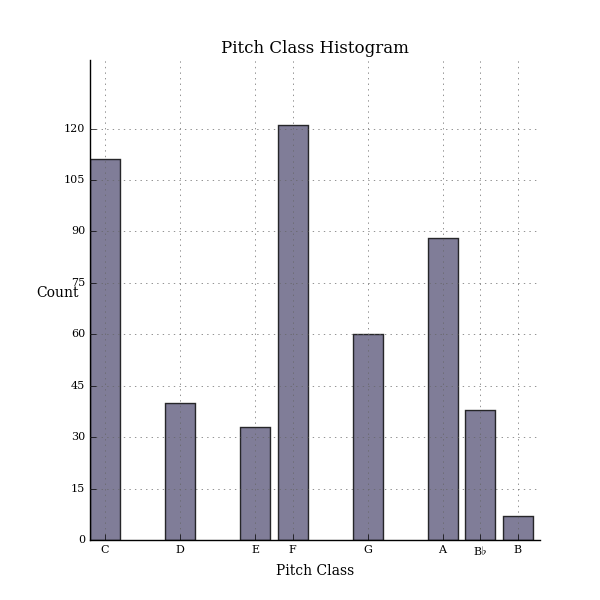
\includegraphics[scale=0.71]{../analysis/bwv1/pitch-class.png}
  \caption{Histograma de \emph{pitch-class} do BWV1. \textbf{Fonte}: Autor}
    \label{fig:pitch-class-bwv1-histogram}
\end{figure}

\begin{figure}[!h]
  \centering
  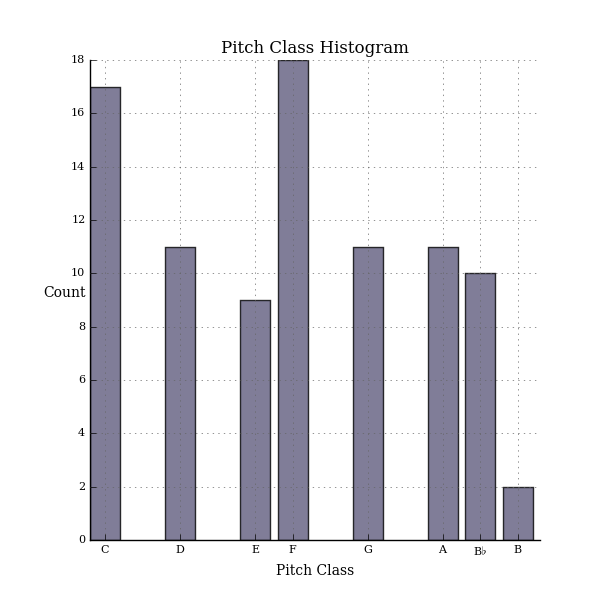
\includegraphics[scale=0.71]{../analysis/bwv1/pitch-class-1.png}
  \caption{Histograma de \emph{pitch-class} da peça Coral \#1. \textbf{Fonte}: Autor}
    \label{fig:pitch-class-bwv1-histogram-2}
\end{figure}

